%%%%%%%%%%%%%%%%%%%%%%%%%%%%%%%%%%%%%%%%%%%%%%%%%%%%%%%%%
% LaTeX Beamer Presentation Generated by AI Researcher
% Paper: "Beyond Labels: Fine-Grained Detection and 
%         Explainable AI for Toxicity in Intimate Dialogues"
%%%%%%%%%%%%%%%%%%%%%%%%%%%%%%%%%%%%%%%%%%%%%%%%%%%%%%%%%

\documentclass[aspectratio=169]{beamer}

\usepackage[utf8]{inputenc}
\usepackage{amsmath}
\usepackage{amsfonts}
\usepackage{amssymb}
\usepackage{graphicx}
\usepackage{booktabs} % For professional tables
\usepackage{caption}  % Add this line for \captionof command

% Choose a theme
\usetheme{Madrid}
\usecolortheme{beaver}

% Adjustments for better presentation
\setbeamertemplate{navigation symbols}{} % Hide navigation symbols
\setbeamertemplate{footline}[frame number] % Show page number
\setbeamerfont{frametitle}{size=\large}
\setbeamerfont{title}{size=\huge}
\setbeamerfont{author}{size=\normalsize}
\setbeamerfont{institute}{size=\small}
\setbeamercovered{transparent} % Make covered items transparent

\title[Toxicity in Intimate Dialogues]{
  Beyond Labels: 
  Fine-Grained Detection and Explainable AI 
  for Toxicity in Intimate Dialogues
}
\author{Nicolò Resta}
\institute{University of Bari, Aldo Moro}
% \date{EVALITA 2025}

\begin{document}

% Title Slide
{
  \setbeamercolor{background canvas}{bg=white}
  \begin{frame}
    \titlepage
  \end{frame}
}

% Outline Slide
\begin{frame}
  \frametitle{Outline}
  \tableofcontents
\end{frame}

% --- SECTION 1: INTRODUCTION ---
\section{Introduction \& Motivation}

\begin{frame}
  \frametitle{The Challenge: Toxicity in Private Conversations}
  \begin{block}{The Problem}
        Detecting toxicity (harassment, abuse) is a critical NLP task for online safety.
        However, most research focuses on \textbf{public platforms} (e.g., Twitter, Reddit, Facebook, Instagram, Youtube).
      \end{block}
      
      \begin{alertblock}{Key Gaps in Private Dialogues}
        \begin{itemize}
          \item \textbf{Data Scarcity:} Sensitive, private nature makes data acquisition nearly impossible.
          \item \textbf{Context is Paramount:} Toxicity is subtle, dyadic, and depends on relational history.
          \item \textbf{Explainability is Crucial:} Simply flagging a chat as "toxic" is insufficient for trust and intervention. We need to answer questions like \textit{how much?} and \textit{why?}
        \end{itemize}
      \end{alertblock}
\end{frame}

\begin{frame}
  \frametitle{Our Contributions}
  
  \begin{enumerate}
    \item \textbf{A Novel Synthetic Data Generation Pipeline} \\
    \pause
    We created a psychologically-grounded pipeline to generate realistic, dyadic \textbf{Italian chats}.
    \begin{itemize}
        \item Annotated with fine-grained, \textit{message-level continuous toxicity scores} [-1, 1].
        \item Includes \textit{human-readable narrative explanations} for chat dynamics.
    \end{itemize}
    \pause
    \item \textbf{A Comprehensive Empirical Study} \\
    \pause
    We conducted experiments across three distinct tasks:
    \begin{itemize}
        \item Chat-Level Classification (Binary \& Multiclass)
        \item Message-Level Regression
        \item Abstractive Explanation Generation
    \end{itemize}
    \pause
    \item \textbf{A Rigorous Comparative Analysis} \\
    \pause
    We statistically compared traditional ML models vs. transformer architectures, revealing key insights about the task's inherent limitations.
  \end{enumerate}
\end{frame}

\section{Dataset Preparation}

% \begin{frame}
%   \frametitle{A 3-Phase Synthetic Data Pipeline: Phase 1, Personas Generation}
%   LLM acts as a psychologist creating detailed profiles:
%   \begin{itemize}
%     \item Demographics: Name, Age, Gender/Pronouns, Occupation, Location, Geographical Context and Family structure
%     \item Core Personality Traits: Big Five (OCEAN), Attachment styles, Emotional triggers, Defensive Mechanisms, Communication Styles ...
%     \item Contextual Background: Personal history, Motivations, Goals, Fears ...
%   \end{itemize}
% \end{frame}

% \begin{frame}
% \end{frame}

\begin{frame}
    \frametitle{A 3-Phase Synthetic Data Pipeline}
    \textbf{Phase 1, Personas Generation:}
    \begin{itemize}
        \item LLM acts as a psychologist.
        \item Creates detailed profiles: Big Five traits (OCEAN), Attachment styles, Emotional triggers, Personal history, Motivations, Defensive Mechanisms and so on ...
    \end{itemize}
    \pause
    \textbf{Phase 2, Chat Generation:}
    \begin{itemize}
        \item Simulates chats across 7 relationship stages (e.g., initiation, exploration ...).
        \item Controlled toxicity by targeting specific \textbf{mean} and \textbf{std. dev.} for message scores.
        \item Each message annotated with a polarity score in $[-1, 1]$.
    \end{itemize}
    \pause
    \textbf{Phase 3, Explanation Generation:}
    \begin{itemize}
        \item LLM acts as a communication expert.
        \item Generates a narrative rationale explaining the toxic or healthy dynamics of the entire chat.
    \end{itemize}

    \pause
    \begin{alertblock}{Result}
        A rich, nuanced dataset grounded in psychological plausibility, tailored for fine-grained analysis and explainability.
    \end{alertblock}
\end{frame}

\begin{frame}
  \frametitle{Preparing the Final Dataset for Experiments}
  
  \begin{block}{Filtering and Cleaning}
    After regex-parsing, filtering (e.g., max length 512 tokens) and cleaning (e.g. converting emojis to text), we obtained \textbf{1809} conversations.
  \end{block}

  \begin{columns}
    \pause
    \begin{column}[T]{0.45\textwidth}
      \begin{block}{Labeling Scheme for Classification}
        \begin{itemize}
            \item \textbf{Aggregation:} Chat label is determined by the class of the \textit{minimum} user-average score.
            \item \textbf{Multiclass:}
            \begin{itemize}
                \item Toxic: $[-1, -0.35)$
                \item Neutral: $[-0.35, 0.35]$
                \item Healthy: $(0.35, 1]$
            \end{itemize}
            \item \textbf{Binary:} Toxic vs. Non-Toxic (Neutral + Healthy).
        \end{itemize}
      \end{block}
    \end{column}
    \pause
    \begin{column}[T]{0.45\textwidth}
      \begin{block}{Dataset Structures}
        \begin{itemize}
            \item \textbf{Classification}: Each sample consists of a textual chat + chat-level label (binary/multiclass).
            \item \textbf{Regression}: Each sample consists of a target message, its message-level score and the full chat as context.
        \end{itemize}
      \end{block}
    \end{column}
  \end{columns}
  
\end{frame}

\begin{frame}
  \frametitle{Dataset Distribution}
  \centering
  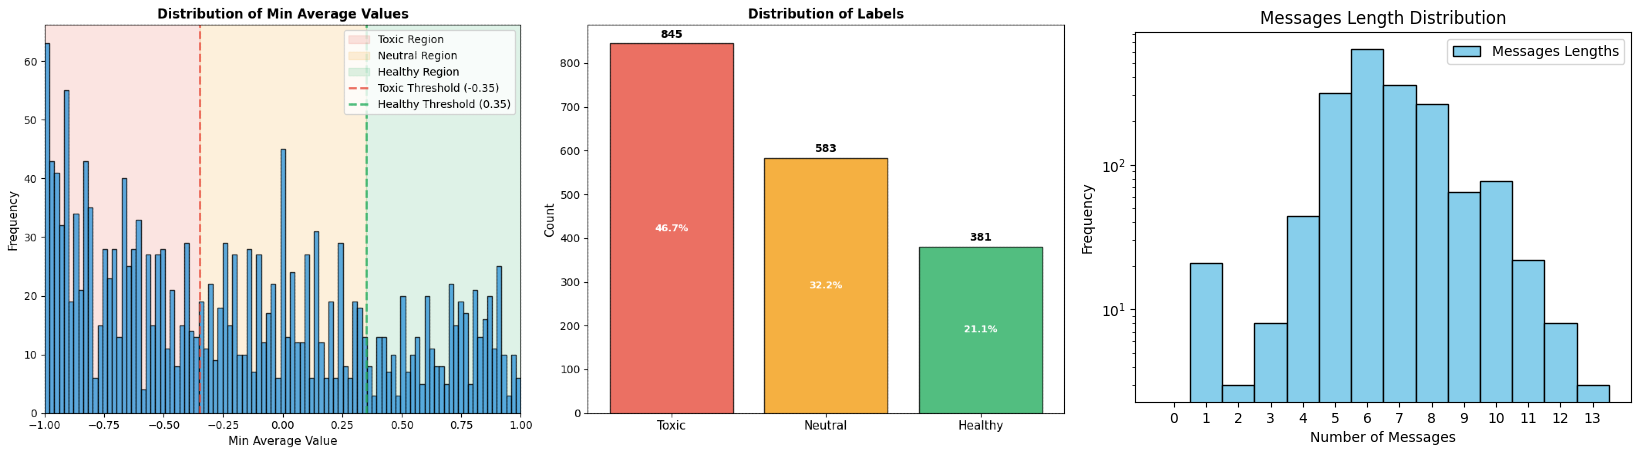
\includegraphics[width=\textwidth]{rsc/multiclass_distributions.png}
  % \captionof{figure}{Multiclass label distribution.}
\end{frame}

% --- SECTION 3: EXPERIMENTS ---
\section{Experiments}

% \begin{frame}
%   \frametitle{Chat-Level Classification}

%   \begin{block}{Classic Models (LR, SVC, NB)}
%     \begin{itemize}
%       \item NLP Pipeline: Tokenization, POS filtering, NER-based anonymization.
%       \item Normalization: Stemming vs. Lemmatization.
%       \item Vectorization: CountVectorizer (NB) and TfidfVectorizer (LR, SVC).
%     \end{itemize}
%   \end{block}
  
%     \pause
%     \begin{block}{BERT Models (Checkpoint: \texttt{dbmdz/bert-base-italian-cased})}
%     \begin{itemize}
%       \item BERT: \texttt{[CLS]} + all messages concatenated.
%       \item BERT-ST: \texttt{[CLS]} + messages separated by \texttt{[SEP]} + token-type IDs.
%     \end{itemize}
%   \end{block}
% \end{frame}

\begin{frame}
  \frametitle{All Models Used}

  \begin{block}{Classic Machine Learning Models}
    For classification task:
    \begin{itemize}
      \item Tokenization
      \item POS filtering: Keep only NOUNs, VERBs, ADJs, ADVs, PRONs, AUXs and INTJs.
      \item NER-based anonymization: Replace PERSON, ORG and LOC.
      \item Normalization: Stemming vs. Lemmatization.
      \item Vectorization + Models: CountVectorizer (NB) and TfidfVectorizer (LR, SVC).
    \end{itemize}
  \end{block}
  
    \pause
    \begin{block}{Transformer Models}
    \begin{itemize}
      \item BERT: \texttt{dbmdz/bert-base-italian-cased} for both classification and regression tasks
      \item BART: \texttt{morenolq/bart-it} for explanation task
    \end{itemize}
  \end{block}
\end{frame}

\begin{frame}
  \frametitle{Cost-Sensitive Prediction Model Variants}
  \begin{itemize}
    \item Logistic Regression and Naive Bayes were also wrapped in a \texttt{CostSensitiveClassifier} to make lowest-cost predictions.
    \item These models were trained and evaluated as standalone models for comparisons.
    \item Cost matrix was defined based on the psychological severity of misclassifications:

    \[
    M =
    \begin{bmatrix}
      0 & 8 & 16 \\
      8 & 0 & 1 \\
      16 & 4 & 0 \\
    \end{bmatrix}
    \]
  \end{itemize}
\end{frame}

\begin{frame}
  \frametitle{BERT Input Formatting Variants for Chat-Level Classification}
  \small
    \textbf{BERT Input (Simple Concatenation):}
    \begin{center}
      \begin{tabular}{|c|c|c|c|c|c|c|c|c|c|}
        \hline
        \texttt{[CLS]} & \texttt{User} & \texttt{A:} & \texttt{msg1} & \texttt{User} & \texttt{B:} & \texttt{msg2} & \texttt{User} & \texttt{A:} & \texttt{msg3} \\
        \hline
      \end{tabular}
    \end{center}
    
    \vspace{0.5cm}
    \textbf{BERT-ST Input (Structured with Speaker Information):}
    \begin{center}
      \resizebox{\textwidth}{!}{%
        \begin{tabular}{|c|c|c|c|c|c|c|c|c|c|c|c|c|}
          \hline
          \texttt{[CLS]} & \texttt{User} & \texttt{A:} & \texttt{msg1} & \texttt{[SEP]} & \texttt{User} & \texttt{B:} & \texttt{msg2} & \texttt{[SEP]} & \texttt{User} & \texttt{A:} & \texttt{msg3} & \texttt{[SEP]} \\
          \hline
          \multicolumn{12}{c}{\scriptsize Token-type IDs:} \\
          \hline
          0 & 0 & 0 & 0 & 0 & 1 & 1 & 1 & 1 & 0 & 0 & 0 & 0 \\
          \hline
        \end{tabular}%
      }
    \end{center}
    
    \vspace{0.3cm}
    \begin{block}{Token-Type IDs}
      \begin{itemize}
        \item Token-type IDs distinguish messages from different users.
        \item Each user's messages are separated by special tokens (\texttt{[SEP]}).
      \end{itemize}
    \end{block}
\end{frame}

% \begin{frame}
%   \frametitle{Message-Level Regression}
  
%   \begin{block}{BERT Models (Checkpoint: \texttt{dbmdz/bert-base-italian-cased})}
%     \begin{itemize}
%       \item BERT-M: Full chat as context, target message wrapped in \texttt{[SEP]}, distinguished with token-type IDs.
%       \item BERT-MU: Role-aware variant of BERT-M with additional learned user embeddings.
%     \end{itemize}
%   \end{block}
% \end{frame}

\begin{frame}
  \frametitle{BERT Input Formatting Variants for Message-Level Regression 1/2}
  \small
    \textbf{BERT-M Input (Target Message Highlighted):}
    \begin{center}
      \resizebox{\textwidth}{!}{%
        \begin{tabular}{|c|c|c|c|c|c|c|c|c|c|c|c|c|c|c|}
          \hline
          \texttt{[CLS]} & \texttt{User} & \texttt{A:} & \texttt{msg1} & \texttt{[SEP]} &\texttt{User} & \texttt{B:} & \texttt{msg2} & \texttt{[SEP]} & \texttt{User} & \texttt{A:} & \texttt{msg3} & \texttt{User} & \texttt{B:} & \texttt{msg4} \\
          \hline
          \multicolumn{15}{c}{\scriptsize Token-type IDs:} \\
          \hline
          1 & 0 & 0 & 0 & 1 & 1 & 1 & 1 & 1 & 0 & 0 & 0 & 0 & 0 & 0 \\
          \hline
        \end{tabular}%
      }
    \end{center}
    
    \vspace{0.3cm}
    \begin{block}{Token-Type IDs}
      \begin{itemize}
        \item Token-type IDs distinguish target and contextual tokens.
        \item The target message is isolated between two special tokens (\texttt{[SEP]}).
      \end{itemize}
    \end{block}
\end{frame}

\begin{frame}
  \frametitle{BERT Input Formatting Variants for Message-Level Regression 2/2}

  \small
    \textbf{BERT-MU Input (With Learned User Embeddings):}
    \begin{center}
      \resizebox{\textwidth}{!}{%
        \begin{tabular}{|c|c|c|c|c|c|c|c|c|c|c|c|c|c|c|}
          \hline
          \texttt{[CLS]} & \texttt{User} & \texttt{A:} & \texttt{msg1} & \texttt{[SEP]} &\texttt{User} & \texttt{B:} & \texttt{msg2} & \texttt{[SEP]} & \texttt{User} & \texttt{A:} & \texttt{msg3} & \texttt{User} & \texttt{B:} & \texttt{msg4} \\
          \hline
          \multicolumn{15}{c}{\scriptsize Token-type IDs:} \\
          \hline
          1 & 0 & 0 & 0 & 1 & 1 & 1 & 1 & 1 & 0 & 0 & 0 & 0 & 0 & 0 \\
          \hline
          \multicolumn{15}{c}{\scriptsize User-type IDs:} \\
          \hline
          $0$ & $1$ & $1$ & $1$ & $0$ & $0$ & $0$ & $0$ & $0$ & $1$ & $1$ & $1$ & $0$ & $0$ & $0$ \\
          \hline
        \end{tabular}%
      }
    \end{center}
    
    \vspace{0.3cm}
    \begin{block}{User-Type IDs}
      \begin{itemize}
        \item Each token also receives a learned user embedding.
        \item This allows the model to capture user-specific communication styles and patterns.
      \end{itemize}
    \end{block}
\end{frame}

\begin{frame}
  \frametitle{Rigorous Evaluation Protocol for Classification/Regression}
  
  \begin{alertblock}{Nested Cross-Validation}
    To get an unbiased performance estimate and tune hyperparameters simultaneously.
    \begin{itemize}
      \item \textbf{Outer Loop (5-fold):} For robust performance estimation.
      \item \textbf{Inner Loop (3-fold):} For hyperparameter tuning (\texttt{GridSearchCV}) (only for ML models).
    \end{itemize}
  \end{alertblock}
  
  \begin{block}{Preventing Data Leakage}
    \textbf{\texttt{GroupKFold}} was used in both loops, ensuring all chats from the same couple remain in the same fold. This is crucial for valid results.
  \end{block}
  
  \begin{block}{Statistical Analysis}
    We computed \textbf{means}, \textbf{std. dev.}, \textbf{95\% confidence intervals}, and conducted \textbf{paired t-tests} on the outer fold scores to determine if performance differences were statistically significant.
  \end{block}
\end{frame}

\begin{frame}
  \frametitle{Evaluation Metrics Across All Tasks}
  \begin{columns}[T]
    \begin{column}{0.32\textwidth}
      \begin{block}{Classification}
        \small
        \begin{itemize}
          \item \textbf{Accuracy}: Ratio of correct predictions
          \item \textbf{Precision}: Accuracy of positive predictions
          \item \textbf{Recall}: Ability to find all positives
          \item \textbf{F1-Score}: Harmonic mean of precision/recall
          \item \textbf{Misclassification Cost}: Custom penalty based on psychological severity (multiclass only)
        \end{itemize}
      \end{block}
    \end{column}
    
    \begin{column}{0.32\textwidth}
      \begin{block}{Regression}
        \small
        \begin{itemize}
          \item \textbf{MAE}: Average absolute error, outlier-robust
          \item \textbf{RMSE - MSE}: Root mean squared error, penalizes large errors
          \item \textbf{Correlation}: Linear relationship strength
          \item \textbf{R-MAE/R-RMSE/R-MSE}: Relative to naive baseline
        \end{itemize}
      \end{block}
    \end{column}
    
    \begin{column}{0.32\textwidth}
      \begin{block}{Explanation Generation}
        \small
        \begin{itemize}
          \item \textbf{ROUGE-1/2}: N-gram overlap (unigrams/bigrams)
          \item \textbf{ROUGE-L}: Longest common subsequence
          \item \textbf{BLEU}: N-gram precision-focused
          \item \textbf{BERTScore}: Semantic similarity using BERT embeddings. Provides P/R/F1 for robust semantic evaluation
        \end{itemize}
      \end{block}
    \end{column}
  \end{columns}
\end{frame}

% \begin{frame}
%   \frametitle{Evaluation Metrics: Classification}
%   \begin{itemize}
%     \item \textbf{Accuracy}: The ratio of correctly predicted instances to the total instances. Can be misleading for imbalanced datasets.
%     \item \textbf{Precision}: Measures the accuracy of positive predictions. Answers: "Of all instances predicted as positive, how many were correct?"
%     \item \textbf{Recall}: Measures the model's ability to identify all relevant instances. Answers: "Of all actual positive instances, how many did the model correctly predict?"
%     \item \textbf{F1-Score}: The harmonic mean of Precision and Recall, providing a single score that balances both.
%     \begin{itemize}
%         \item \textit{Weighted F1} is used to account for class imbalance.
%     \end{itemize}
%     \item \textbf{Misclassification Cost}: A custom metric for the \textbf{multiclass task only} that assigns different penalties to different types of errors based on their psychological severity. The goal is to minimize this cost.
%   \end{itemize}
% \end{frame}

% \begin{frame}
%   \frametitle{Evaluation Metrics: Regression}
%   \begin{itemize}
%     \item \textbf{Mean Absolute Error (MAE)}: The average of the absolute differences between predicted and actual values. It's easy to interpret and less sensitive to outliers.
%     \item \textbf{Root Mean Squared Error (RMSE)}: The square root of the average of squared differences. It penalizes larger errors more heavily than MAE.
%     \item \textbf{Correlation Coefficient}: Measures the strength and direction of the linear relationship between predicted and actual scores. A value of 1 indicates a perfect positive correlation.
%     \item \textbf{Relative Metrics (R-MAE, R-RMSE)}: These metrics compare the model's error to that of a naive baseline model that always predicts the average score. A value below 1 indicates the model is better than the baseline.
%   \end{itemize}
% \end{frame}

% \begin{frame}
%   \frametitle{Evaluation Protocol: Explanation Generation}
%   First 64\% training, 16\% validation, 20\% test split, then:
%   \begin{itemize}
%     \item \textbf{ROUGE (Recall-Oriented Understudy for Gisting Evaluation)}: Measures the overlap of n-grams, word sequences, and word pairs between the generated and reference texts.
%     \begin{itemize}
%         \item \textit{ROUGE-1/2}: Overlap of unigrams/bigrams.
%         \item \textit{ROUGE-L}: Longest common subsequence.
%     \end{itemize}
%     \item \textbf{BLEU (Bilingual Evaluation Understudy)}: Measures how many n-grams in the generated text also appear in the reference text. It focuses on precision.
%     \item \textbf{BERTScore}: Uses contextual embeddings from BERT to compare the semantic similarity between tokens in the generated and reference texts.
%     \begin{itemize}
%         \item It provides \textit{Precision}, \textit{Recall}, and an \textit{F1-Score}, offering a more robust measure of semantic equivalence than n-gram overlap.
%     \end{itemize}
%   \end{itemize}
% \end{frame}

\begin{frame}
  \frametitle{Hyperparameters Space}
  \begin{columns}[T]
    \begin{column}{0.45\textwidth}
      \begin{table}
        \resizebox{\textwidth}{!}{%
          \begin{tabular}{lll}
            \hline
            \textbf{Component} & \textbf{Hyperparameter} & \textbf{Values} \\
            \hline
            \texttt{Count/Tfidf} & \texttt{ngram\_range} & (1, 1), (1, 2), (1, 3) \\
            \texttt{Vectorizer} & \texttt{min\_df} & 3, 8, 20 \\
            & \texttt{max\_df} & 0.9, 0.95, 0.99 \\
            \hline
            Multinomial NB & \texttt{alpha} & 0.1, 0.5, 1.0, 2.0 \\
            \hline
            Logistic Regression & \texttt{C} & 0.1, 1.0, 10.0 \\
            & \texttt{max\_iter} & 1000, 2000 \\
            \hline
            BERT & n. Max. Epochs & 20 \\
            & Learning Rate & 3e-5 \\
            & Batch Size & 32 \\
            & Grad. Accum. Steps & 4 \\
            & Weight Decay & 0.001 \\
            & Warmup Percentage & 0.1 \\
            & Early Stopping & Patience: 4 \\
            & LR Scheduler & Reduce on Plateau \\
            & (Factor: 0.5, & Patience: 2) \\
          \hline
          \end{tabular}%
        }
      \end{table}
    \end{column}
    \begin{column}{0.45\textwidth}
      \begin{table}
        \vspace{0pt}
        \resizebox{\textwidth}{!}{%
          \begin{tabular}{lll}
            \hline
            \textbf{Component} & \textbf{Hyperparameter} & \textbf{Values} \\
            \hline
              BART & n. Max. Epochs & 20 \\
              & Learning Rate & 3e-5 \\
              & Batch Size & 4 \\
              & Grad. Accum. Steps & 8 \\
              & Weight Decay & 0.01 \\
              & Warmup Percentage & 0.1 \\
              & LR Scheduler & Linear with Warmup \\
            \hline
          \end{tabular}%
        }
      \end{table}
    \end{column}
  \end{columns}
\end{frame}

% \begin{frame}
%   \frametitle{Hyperparameters Space 2/2}
  
% \end{frame}

\begin{frame}
  \frametitle{Best Model Selection Criteria}
  \begin{block}{Chat-Level Classification Tasks}
    \begin{itemize}
      \item Binary: Maximize \textbf{Weighted F1-score}.
      \item Multiclass: Minimize \textbf{Chat-Level Misclassification Cost} of chat-level predictions.
    \end{itemize}
  \end{block}
  \begin{block}{Message-Level Regression Task}
    Minimize \textbf{Message-Level Misclassification Cost} of aggregated message-level predictions.
  \end{block}
  \begin{block}{Explanation Generation Task}
    Maximize \textbf{BERTScore F1} between generated and reference explanations.
  \end{block}
\end{frame}

% --- SECTION 4: RESULTS ---
\section{Results}

\begin{frame}
  \frametitle{Finding 1: A Performance Plateau in Classification (Multiclass)}
  \begin{columns}[T]
    \begin{column}{0.45\textwidth}
      \small

    \begin{table}[H]
        \centering
        % \caption{Model Performance by Cost (Best to Worst)}
        \resizebox{\textwidth}{!}{%
          \begin{tabular}{@{}lcc@{}}
              \toprule
              \textbf{Model} & \textbf{Weighted F1} & \textbf{Cost} \\
              \midrule
              \textbf{BERT-M} & $0.78 \pm 0.04\,[0.72, 0.83]$ & $0.10 \pm 0.02\,[0.07, 0.12]$\\
              BERT & $0.77 \pm 0.03\,[0.72, 0.81]$ & $0.10 \pm 0.02\,[0.07, 0.13]$\\
              BERT-MU & $0.77 \pm 0.05\,[0.71, 0.84]$ & $0.10 \pm 0.02\,[0.07, 0.13]$\\
              PosNerStem-SVC & $0.77 \pm 0.03\,[0.73, 0.80]$ & $0.11 \pm 0.01\,[0.09, 0.13]$\\
              PosNerLemma-SVC & $0.77 \pm 0.03\,[0.73, 0.80]$ & $0.11 \pm 0.01\,[0.09, 0.13]$\\
              PosNerStem-LR & $0.76 \pm 0.02\,[0.73, 0.79]$ & $0.11 \pm 0.01\,[0.09, 0.12]$\\
              PosNerLemma-LR & $0.76 \pm 0.02\,[0.73, 0.79]$ & $0.11 \pm 0.01\,[0.09, 0.12]$\\
              BERT-ST & $0.76 \pm 0.04\,[0.70, 0.81]$ & $0.11 \pm 0.02\,[0.08, 0.14]$\\
              PosNerStem-CS\_NB & $0.75 \pm 0.03\,[0.70, 0.79]$ & $0.12 \pm 0.02\,[0.10, 0.15]$\\
              PosNerStem-NB & $0.75 \pm 0.04\,[0.70, 0.80]$ & $0.12 \pm 0.02\,[0.09, 0.15]$\\
              PosNerLemma-CS\_NB & $0.75 \pm 0.03\,[0.70, 0.79]$ & $0.12 \pm 0.02\,[0.10, 0.15]$\\
              PosNerLemma-NB & $0.75 \pm 0.04\,[0.70, 0.80]$ & $0.12 \pm 0.02\,[0.09, 0.15]$\\
              PosNerStem-CS\_LR & $0.73 \pm 0.03\,[0.68, 0.77]$ & $0.12 \pm 0.02\,[0.09, 0.15]$\\
              PosNerLemma-CS\_LR & $0.73 \pm 0.03\,[0.68, 0.77]$ & $0.12 \pm 0.02\,[0.09, 0.15]$\\
              % BERT-M & $0.72 \pm 0.03\,[0.68, 0.76]$ & $0.13 \pm 0.02\,[0.1, 0.15]$\\
              % BERT-MU & $0.71 \pm 0.03\,[0.67, 0.75]$ & $0.13 \pm 0.02\,[0.11, 0.15]$\\
              \bottomrule
          \end{tabular}%
        }
    \end{table}

    \end{column}
    \begin{column}{0.45\textwidth}
      \centering
      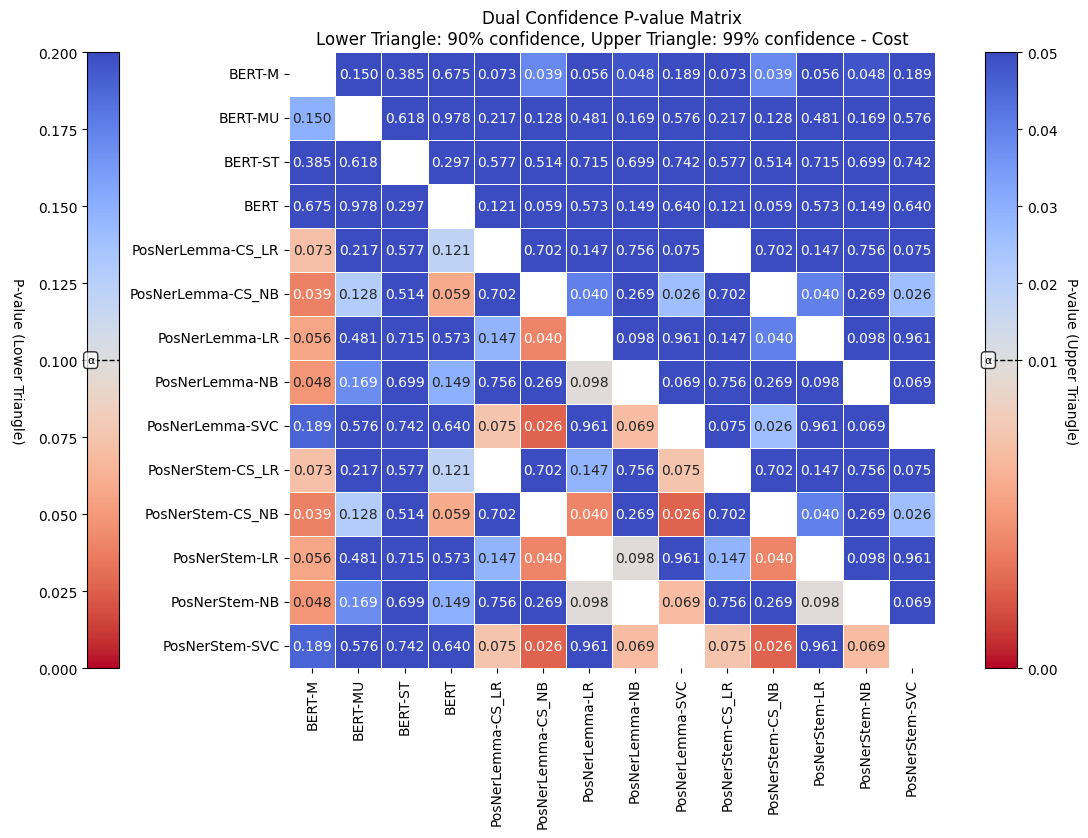
\includegraphics[width=\textwidth]{rsc/multiclass_statistical_tests2.png}
      % \captionof{figure}{\small Paired t-tests show no significant difference among top models (blue = not significant).}
    \end{column}
  \end{columns}
  
  \begin{alertblock}{Interpretation}
    The task's and labeling scheme's inherent \textbf{subjectivity and ambiguity} may have challenged all models equally limiting performances.
  \end{alertblock}
\end{frame}

\begin{frame}
  \frametitle{Finding 1: A Performance Plateau in Classification (Binary)}
  \begin{columns}[T]
    \begin{column}{0.45\textwidth}
      \small
      \begin{table}[H]
        \centering
        % \caption{Model Performance by Weighted F1 Score (Best to Worst)}
        % \resizebox{\textwidth}{!}{%
          \begin{tabular}{@{}lc@{}}
              \toprule
              \textbf{Model} & \textbf{Weighted F1} \\
              \midrule
              \textbf{SVC} & $0.87 \pm 0.03\,[0.83, 0.91]$ \\
              \textbf{BERT} & $0.87 \pm 0.02\,[0.84, 0.90]$ \\
              \textbf{BERT-M} & $0.87 \pm 0.02\,[0.84, 0.90]$ \\
              LR & $0.86 \pm 0.02\,[0.83, 0.90]$ \\
              BERT-ST & $0.86 \pm 0.02\,[0.82, 0.89]$ \\
              BERT-MU & $0.86 \pm 0.03\,[0.82, 0.89]$ \\
              NB & $0.84 \pm 0.03\,[0.81, 0.88]$ \\
              % BERT-M (Message-Level) & $0.84 \pm 0.02\,[0.82, 0.86]$ \\
              % BERT-MU (Message-Level) & $0.83 \pm 0.02\,[0.80, 0.86]$ \\
              \bottomrule
          \end{tabular}
        % }
    \end{table}
    \end{column}
    \begin{column}{0.45\textwidth}
      \centering
      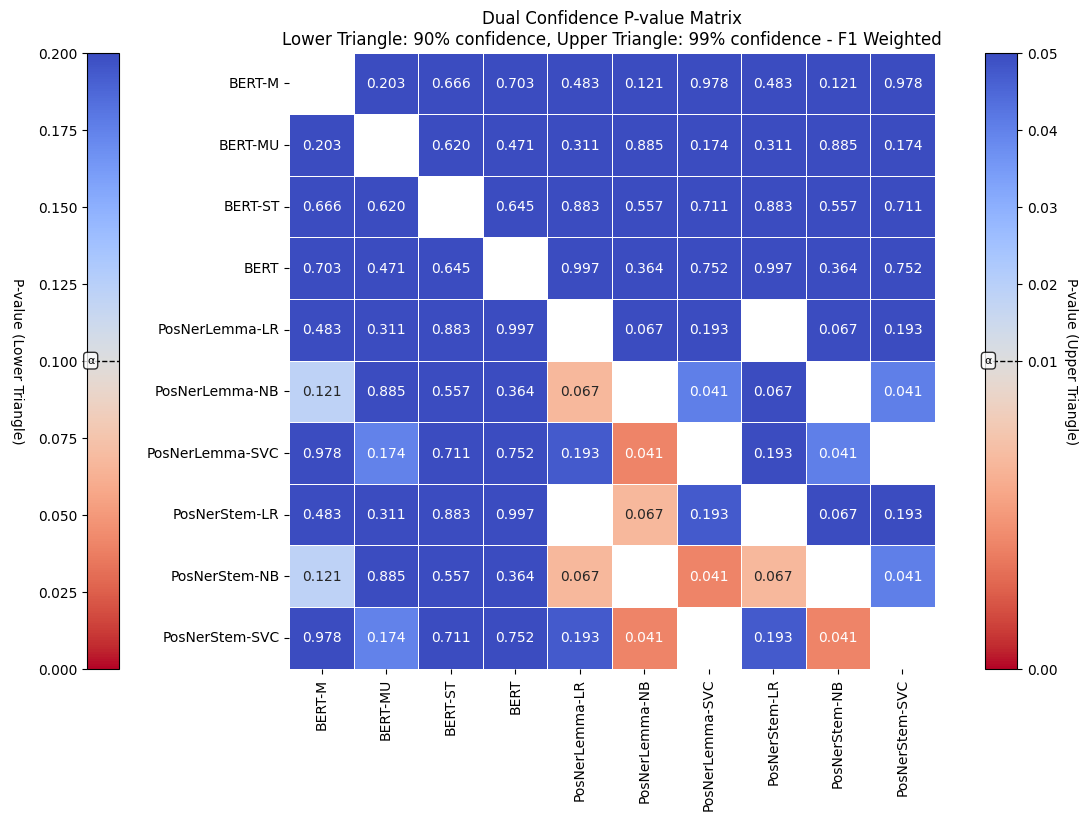
\includegraphics[width=\textwidth]{rsc/binary_statistical_tests2.png}
    \end{column}
  \end{columns}

  \begin{alertblock}{Interpretation}
    Mistakenly introduced dataset latent biases may be learnable up to a certain point, beyond which further complex models yields diminishing returns.
  \end{alertblock}
\end{frame}

% \begin{frame}
%   \frametitle{Finding 1: A Performance Plateau in Classification}
  
%   \begin{block}{Multiclass Classification (toxic, neutral, healthy)}
%     \begin{itemize}
%       \item Top models converge around a \textbf{Weighted F1-score of ~0.78}.
%       \item \alert{Key Finding:} Classic models like \textbf{Logistic Regression} and \textbf{SVC} perform on par with more complex \textbf{BERT} architectures.
%     \end{itemize}
%   \end{block}
  
%   \begin{columns}[T]
%     \begin{column}{0.5\textwidth}
%       \small
%       \begin{tabular}{lcc}
%         \toprule
%         \textbf{Model} & \textbf{Weighted F1} & \textbf{Cost} \\
%         \midrule
%         PosNerStem-LR & $0.76 \pm 0.02$ & $0.11 \pm 0.01$ \\
%         PosNerStem-SVC & $0.77 \pm 0.03$ & $0.11 \pm 0.01$ \\
%         BERT & $0.77 \pm 0.03$ & $0.10 \pm 0.02$ \\
%         \textbf{BERT-M (Reg.)} & $\mathbf{0.78 \pm 0.04}$ & $\mathbf{0.10 \pm 0.02}$ \\
%         \bottomrule
%       \end{tabular}
%     \end{column}
%     \begin{column}{0.5\textwidth}
%       \centering
%       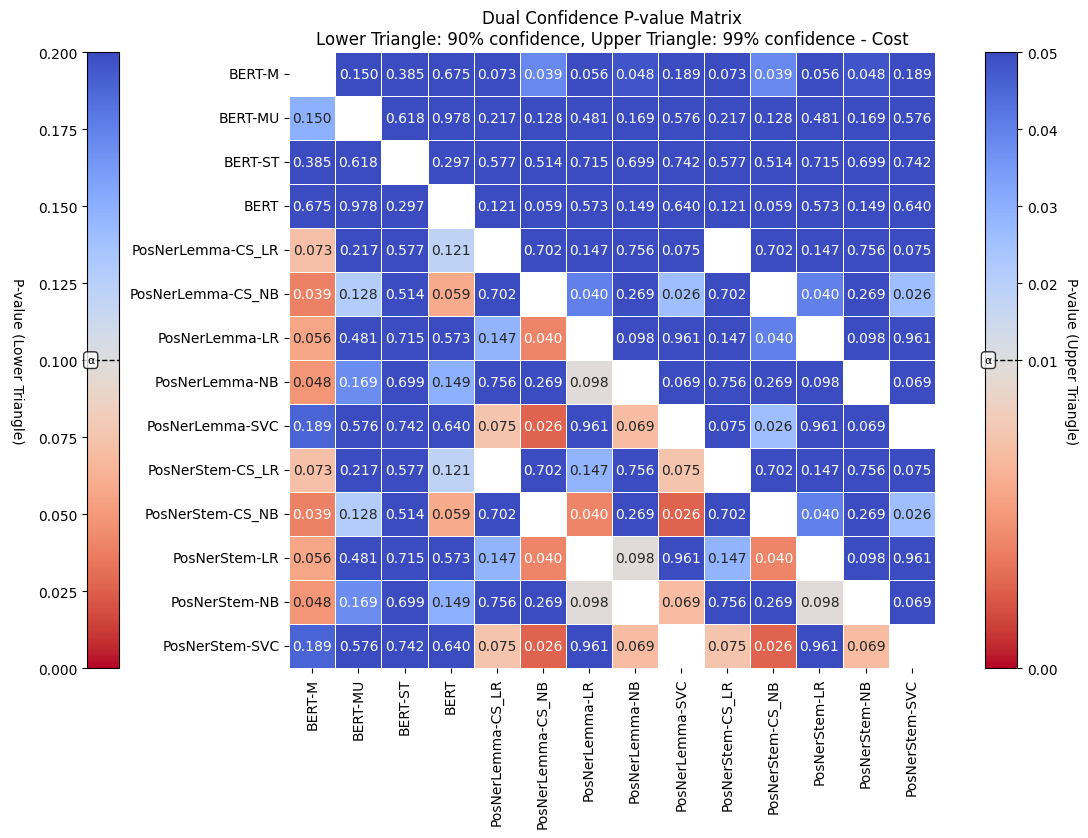
\includegraphics[width=\textwidth]{rsc/multiclass_statistical_tests2.png}
%       \captionof{figure}{\small Paired t-tests show no significant difference among top models (blue = not significant).}
%     \end{column}
%   \end{columns}
  
%   \begin{alertblock}{Interpretation}
%     Performance is likely limited by the task's inherent \textbf{subjectivity and ambiguity}, not model complexity.
%   \end{alertblock}
% \end{frame}

\begin{frame}
  \frametitle{Finding 2: Regression is a Viable Alternative}
  \begin{table}[H]
    \centering
    % \caption{Performance Metrics of Two Models}
    \small % Make the text slightly smaller to fit
    \resizebox{\textwidth}{!}{%
        \begin{tabular}{lcc}
            \toprule
            \textbf{Metric} & \textbf{BERT-M} & \textbf{BERT-MU} \\
            \midrule
            Mean Squared Error (MSE) & $0.1367 \pm 0.0168 \ [0.1159, 0.1576]$ & $0.1423 \pm 0.0194 \ [0.1182, 0.1664]$ \\
            Mean Absolute Error (MAE) & $0.2656 \pm 0.0216 \ [0.2388, 0.2925]$ & $0.2695 \pm 0.0223 \ [0.2419, 0.2972]$ \\
            Root Mean Squared Error (RMSE) & $0.3692 \pm 0.0225 \ [0.3413, 0.3972]$ & $0.3765 \pm 0.0257 \ [0.3446, 0.4085]$ \\
            Correlation Coefficient & $0.8335 \pm 0.0264 \ [0.8007, 0.8663]$ & $0.8254 \pm 0.0266 \ [0.7923, 0.8584]$ \\
            Relative MSE (R-MSE) & $0.3205 \pm 0.0391 \ [0.2720, 0.3691]$ & $0.3338 \pm 0.0467 \ [0.2758, 0.3918]$ \\
            Relative MAE (R-MAE) & $0.4618 \pm 0.0372 \ [0.4156, 0.5080]$ & $0.4687 \pm 0.0390 \ [0.4203, 0.5171]$ \\
            Relative RMSE (R-RMSE) & $0.5653 \pm 0.0342 \ [0.5229, 0.6078]$ & $0.5766 \pm 0.0406 \ [0.5261, 0.6270]$ \\
            Message-Level Binary Weighted F1 & $0.84 \pm 0.02\,[0.82, 0.86]$ & $0.83 \pm 0.02\,[0.80, 0.86]$ \\
            Message-Level Multiclass Weighted F1 & $0.72 \pm 0.03\,[0.68, 0.76]$ & $0.71 \pm 0.03\,[0.67, 0.75]$ \\
            Message-Level Multiclass Cost & $0.13 \pm 0.02\,[0.10, 0.15]$ & $0.13 \pm 0.02\,[0.11, 0.15]$ \\
            \bottomrule
        \end{tabular}%
    }
  \end{table}
  \begin{alertblock}{Interpretation}
    Models are effective at capturing the nuances of toxicity in messages. They also achieved competitive classification performances, validating the fine-grained approach.
  \end{alertblock}
\end{frame}

% \begin{frame}
%     \frametitle{Finding 2: Regression is a Viable Alternative}
    
%     \begin{block}{Message-Level Regression Performance}
%         Both BERT regression models accurately predict continuous toxicity scores.
%         \begin{itemize}
%             \item \textbf{Correlation Coefficient > 0.82} with ground truth.
%             \item Substantial improvement over a naive baseline (e.g., R-MAE ~0.46).
%             \item The simpler \textbf{BERT-M} model slightly outperformed the role-aware \textbf{BERT-MU}.
%         \end{itemize}
%     \end{block}

%     \begin{table}
%         \centering
%         \caption{Message-Level Regression Metrics}
%         \small
%         \begin{tabular}{lcc}
%             \toprule
%             \textbf{Metric} & \textbf{BERT-M} & \textbf{BERT-MU} \\
%             \midrule
%             Correlation Coefficient & $\mathbf{0.8335 \pm 0.0264}$ & $0.8254 \pm 0.0266$ \\
%             Relative MAE (R-MAE) & $\mathbf{0.4618 \pm 0.0372}$ & $0.4687 \pm 0.0390$ \\
%             \bottomrule
%         \end{tabular}
%     \end{table}

%     \begin{alertblock}{Connecting Regression to Classification}
%         When aggregating regression scores to produce chat-level labels, the \textbf{BERT-M} model achieves top-tier classification performance (\textbf{0.78 F1} multiclass, \textbf{0.87 F1} binary), proving the validity of the fine-grained approach. However, it does not offer a \textit{statistically significant} advantage over direct classification.
%     \end{alertblock}
% \end{frame}

\begin{frame}
  \frametitle{Finding 3: Promising Results in Explainability}
  
  % \begin{block}{Abstractive Explanation Generation}
  %   The BART model was trained to generate narrative summaries of chat dynamics.
  % \end{block}
  
  \begin{columns}[T]
    \begin{column}{0.35\textwidth}
      \begin{table}
        % \centering
        % \caption{Explanation Generation Test Metrics}
        \begin{tabular}{lr}
          \toprule
          \textbf{Metric} & \textbf{Value} \\
          \midrule
          \textbf{BERTScore (F1)} & \textbf{0.77} \\
          BERTScore (Precision) & 0.77 \\
          BERTScore (Recall) & 0.76 \\
          ROUGE-1 & 0.56 \\
          ROUGE-2 & 0.21 \\
          ROUGE-L & 0.25 \\
          BLEU & 0.20 \\
          \bottomrule
        \end{tabular}
      \end{table}
    \end{column}
    \begin{column}{0.55\textwidth}
      \begin{alertblock}{Interpretation}
        \begin{itemize}
            \item \textbf{High BERTScore F1 (0.77)} indicates strong \textit{semantic similarity} between generated and reference explanations. The model captures the correct meaning.
            \item Lower n-gram scores (ROUGE-2, BLEU) are expected in abstractive tasks with high linguistic variability.
        \end{itemize}
      \end{alertblock}
    \end{column}
  \end{columns}
  \begin{block}{Considerations}
    Overall the model can generate coherent and contextually relevant rationales, a crucial step towards trustworthy AI.
  \end{block}
\end{frame}


% --- SECTION 5: CONCLUSION ---
\section{Conclusion \& Future Work}

\begin{frame}
  \frametitle{Conclusions}
  
  \begin{itemize}
    \item We introduced a novel, psychologically-grounded pipeline for generating rich synthetic data for toxicity analysis in intimate dialogues.
    \pause
    \item Our key finding is a \textbf{performance plateau}: a diverse range of models (from LR to BERT) achieve statistically similar peak F1-scores (~0.78 multiclass, ~0.87 binary).
    \pause
    \item This suggests performance is currently bottlenecked by the \textbf{task's inherent ambiguity} and data characteristics, rather than model complexity.
    \pause
    \item The fine-grained regression approach demonstrated promising competitively performances on classification tasks when its outputs are aggregated.
    \pause
    \item Our BART model demonstrates promising capabilities for generating \textbf{semantically relevant explanations}, paving the way for more transparent systems.
  \end{itemize}
\end{frame}

\begin{frame}
  \frametitle{Future Work}
  
  Our ongoing research focuses on four key areas:
  
  \begin{enumerate}
    \item \textbf{Enhancing Data Generation \& Quality Assessment} \\
    Refining the pipeline with automated quality metrics and exploring multi-agent (e.g., critic/generator) frameworks to improve realism.

    \item \textbf{Interdisciplinary Collaboration} \\
    Integrating professional psychologists into the research team to improve psychological fidelity and validate model behaviors.
    
    \item \textbf{Real-World Validation} \\
    Deploying a public demo to collect user feedback, bridging the "sim-to-real" gap and testing model generalization.
    
    \item \textbf{Multi-Task Learning for Enhanced Explainability} \\
    Training a single BART-based model for both regression and explanation generation, using explanation as a form of regularization to learn more robust representations.
  \end{enumerate}
\end{frame}

% Final Slide
\begin{frame}
  \centering
  \Huge Thank You! \\
  \vspace{0.5cm}
  \normalsize
  \textbf{Nicolò Resta} \\
  nicolo.resta@studenti.uniba.it \\
  University of Bari, Aldo Moro \\

\end{frame}

\end{document}